\section{Campos eléctricos}

  \subsection{Propiedades de las cargas eléctricas}
    \PN Propiedades:
    \begin{itemize}
      \item existen dos tipos de cargas eléctricas, \textit{positiva} y \textit{negativa}.
      \item cargas de un mismo signo se repelen y cargas de signos opuestos se atraen.
      \item en un sistema aislado la carga eléctrica siempre se conserva.
      \item las cargas eléctricas siempre se presentan como un entero múltiplo de una cantidad básica de carga $e$.
      \item la carga eléctrica se escribe $q = \pm Ne$ donde $N$ es algún número entero.
      \item el electrón tiene una carga $-e$ y el protón una carga $+e$. El neutrón, no posee carga.
    \end{itemize}

  \subsection{Objetos de carga mediante inducción}
    \begin{itemize}
      \item Los \textbf{conductores} eléctricos son aquellos materiales en los cuales algunos de los electrones son
      libres no están unidos a átomos y pueden moverse con libertad a través del material.
      \item Los \textbf{aislantes} eléctricos son aquellos materiales en los cuales todos los electrones están unidos a
      átomos y no pueden moverse libremente a través del material.
      \item Los \textbf{semiconductores}, tienen propiedades eléctricas que se ubican entre las correspondientes a los
      aislantes y a los conductores.
    \end{itemize}

  \subsection{Ley de Coulomb}
    \PN Al generalizar las propiedades de la fuerza eléctrica entre dos partículas inmóviles con carga, se usa el
    término \textit{carga puntual} que hace referencia a una partícula con carga de tamaño cero.

    \PN Debido a observaciones experimentales es posible encontrar la magnitud de una fuerza eléctrica entre dos cargas
    puntuales establecidas por la \textbf{Ley de Coulomb}:
    \begin{equation*}
      F = k \ \frac{\abs{q_{1}} \abs{q_{2}}}{r^{2}}
    \end{equation*}

    \PN donde k es una constante conocida como constante de Coulomb.

    \PN La fuerza eléctrica, como la fuerza de gravedad, es conservativa.

    \PN La unidad de carga del SI es el \textbf{coulomb (C)}. La constante de Coulomb k en unidades del SI tiene el
    valor:
    \begin{equation*}
      k = 8.987 \ \text{x} \ 10^{9} \ \frac{\text{N} m^{2}}{\text{C}^{2}}
    \end{equation*}

    \PN Además esta constante se expresa como:
    \begin{equation*}
      k = \frac{1}{4 \pi \varepsilon_{0}}
    \end{equation*}

    \PN donde la constante $\varepsilon_{0}$ se conoce como la \textit{permitividad del vacío}, cuyo valor es:
    \begin{equation*}
      \varepsilon_{0} = 8.8542 \ \text{x} \ 10^{-12} \ \frac{\text{C}^{2}}{\text{N} m^{2}}
    \end{equation*}

    \PN La unidad de carga más pequeña, es la carga de un electrón ($-e$) o de un protón ($e$), con una magnitud de:
    \begin{equation*}
      e = 1.60218 \ \text{x} \ 10^{-19} \text{C}
    \end{equation*}

    \PN La ley de Coulomb, expresada en forma vectorial para una fuerza eléctrica ejercida por una carga $q_{1}$ sobre
    una segunda carga $q_{2}$, rescrita como $\vec{F}_{12}$, es
    \begin{equation*}
      \vec{F}_{12} = k \ \frac{q_{1} q_{2}}{r^{2}} \ \hat{r}_{12}
    \end{equation*}

    \PN donde $\hat{r}_{12}$ es un vector unitario dirigido de $q_{1}$ hacia $q_{2}$.
    \begin{figure}[H]
    \centering
      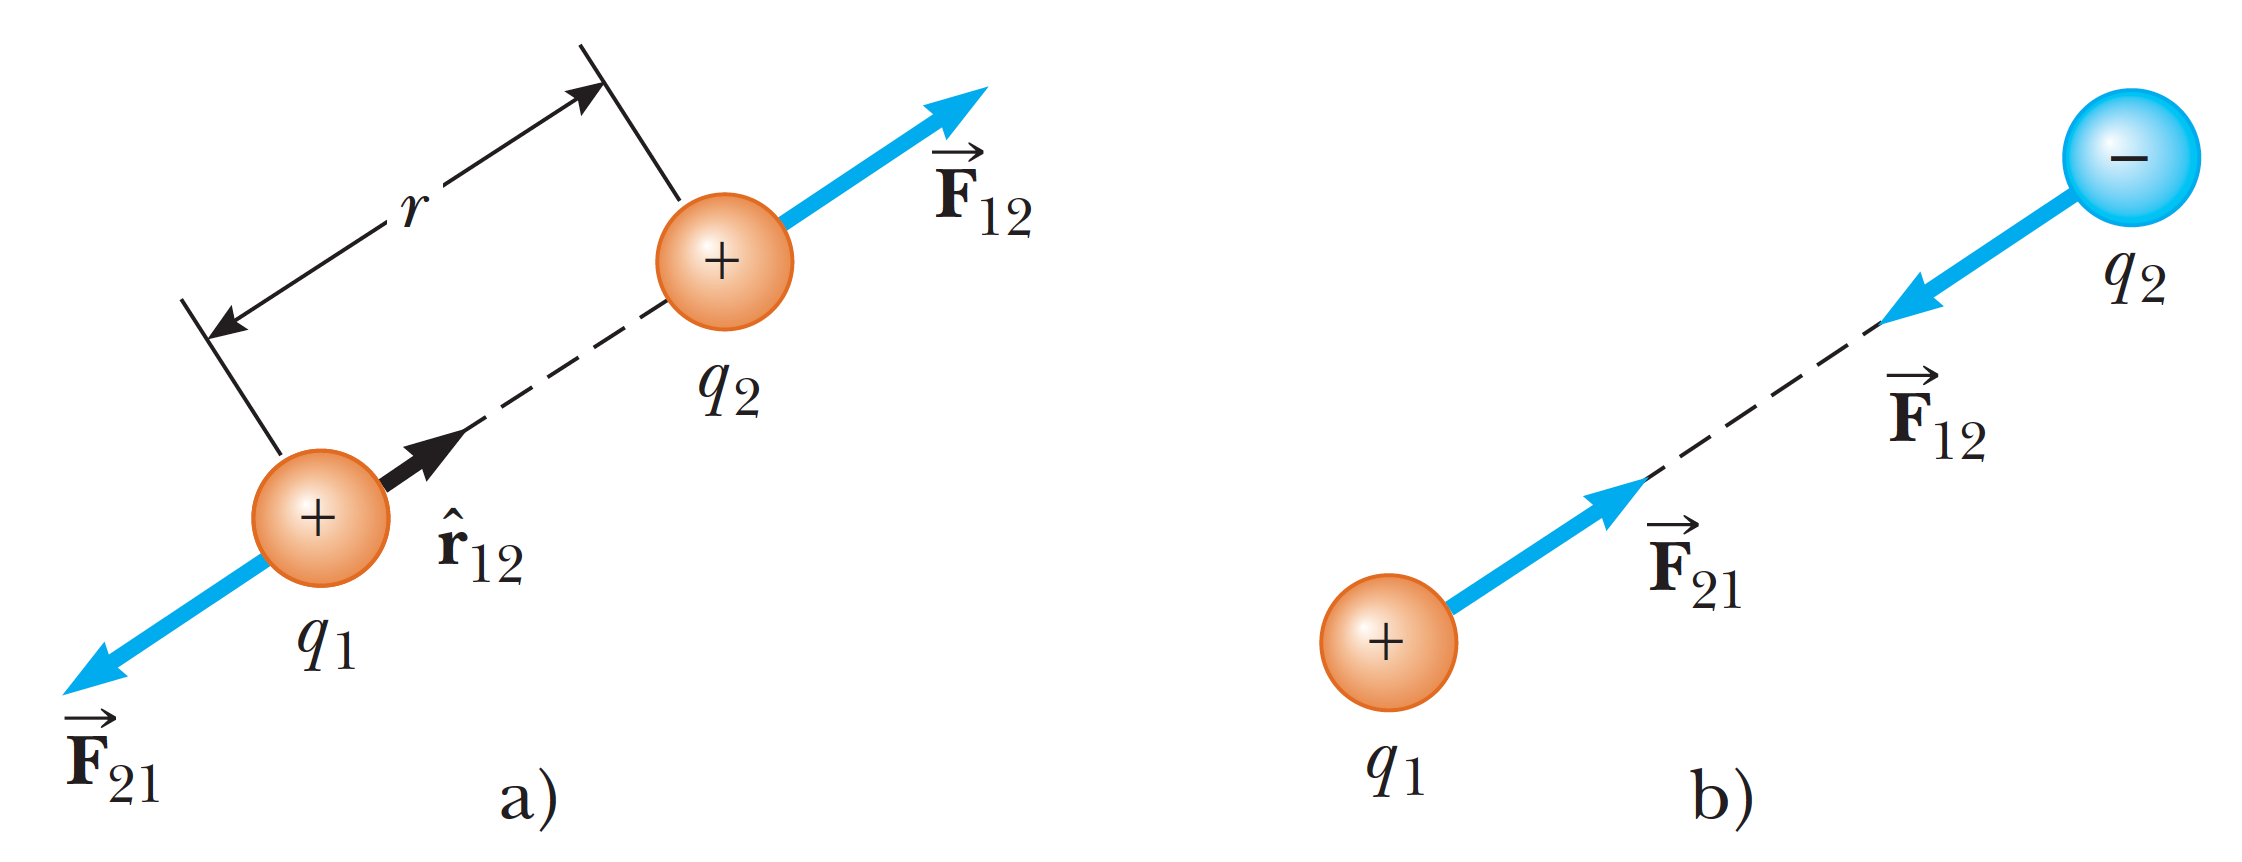
\includegraphics[width=0.5\textwidth]{4/figure_1}
      \caption{Dos cargas puntuales separadas por una distancia $r$ ejercen una fuerza mutua que está determinada por la
      Ley de Coulomb.}
    \end{figure}

    \PN Si $q_{1}$ y $q_{2}$ son del mismo signo, el producto $q_{1} q_{2}$ es positivo. Si $q_{1}$ y $ q_{2}$ son de
    signos opuestos, el producto $q_{1} q_{2}$ es negativo. Estos signos indican la dirección \textit{relativa} de la
    fuerza, pero no la dirección \textit{absoluta}. Un producto negativo indica que se trata de una \textbf{fuerza de
    atracción}, por lo que cada una de las cargas experimenta una fuerza hacia la otra. Un producto positivo indica que
    se trata de una \textbf{fuerza de repulsión} tal que cada carga experimenta una fuerza que la separa de la otra. La
    dirección absoluta de la fuerza sobre una carga depende de la posición de la otra carga.

    \VS
    \PN Cuando hay más de dos cargas presentes, la fuerza resultante de cualquiera de ellas es igual a la suma vectorial
    de las fuerzas ejercidas por las otras cargas individuales. Por ejemplo, si están presentes cuatro cargas, la fuerza
    resultante ejercida por las partículas 2, 3 y 4 sobre la partícula 1 es de
    \begin{equation*}
      \vec{F}_{1} = \vec{F}_{21} + \vec{F}_{31} + \vec{F}_{41}
    \end{equation*}

  \subsection{El campo eléctrico}
    \PN El concepto de campo fue desarrollado por Faraday en relación con las fuerzas eléctricas. En este planteamiento,
    existe un \textbf{campo eléctrico} en la región del espacio que rodea a un objeto con carga: la \textbf{carga
    fuente}. Cuando otro objeto con carga, la \textbf{carga de prueba}, entra en este campo eléctrico, una fuerza
    eléctrica actúa sobre él.

    \VS
    \PN El vector $\vec{E}$ del campo eléctrico en un punto en el espacio se define como la \textbf{fuerza eléctrica}
    $\vec{F}$, que actúa sobre una carga de prueba positiva $q_{0}$ colocada en ese punto, dividida entre la carga de
    prueba
    \begin{equation*}
      \vec{E} \equiv \frac{\vec{F}}{q_{0}}
    \end{equation*}

    \PN El vector $\vec{E}$ está en unidades del SI, newtons por cada coulomb (N/C). Observe que $\vec{E}$ es el campo
    producido por una carga o distribución de carga separada de la carga de prueba; no es el campo producido por la
    propia carga de prueba, además observe que la existencia de un campo eléctrico es una propiedad de su fuente; la
    presencia de una carga de prueba no es necesaria para que el campo exista. La carga de prueba sirve como detector
    del campo eléctrico.

    \VS
    \PN La dirección de $\vec{E}$, es la dirección de la fuerza que experimenta una carga de prueba positiva cuando es
    colocada en el campo; existe un campo eléctrico en un punto si una carga de prueba en dicho punto experimenta una
    fuerza eléctrica.

    \VS
    \PN La fuerza ejercida sobre una partícula con carga $q$ colocada en un campo eléctrico es
    \begin{equation*}
      \vec{F} = q \vec{E}
    \end{equation*}

    \PN Si $q$ es positiva, la fuerza tiene la misma dirección que el campo. Si es negativa, la fuerza y el campo tienen
    direcciones opuestas.

    \VS
    \PN Para determinar la dirección que tiene un campo eléctrico, considere una carga puntual $q$ como carga fuente.
    Esta carga produce un campo eléctrico en todos los puntos del espacio que la rodea. En el punto P, a una distancia
    $r$ de la carga fuente, se coloca una carga de prueba $q_{0}$. Imagine el uso de la carga de prueba para determinar
    la dirección de la fuerza eléctrica y, por lo tanto, la dirección del campo eléctrico. De acuerdo con la ley de
    Coulomb, la fuerza ejercida por $q$ sobre la carga de prueba es
    \begin{equation*}
      \vec{F} = k \ \frac{q q_{0}}{r^{2}} \ \hat{r}
    \end{equation*}

    \PN dónde $\hat{r}$ es un vector unitario con dirección de $q$ hacia $q_{0}$.

    \begin{figure}[H]
    \centering
      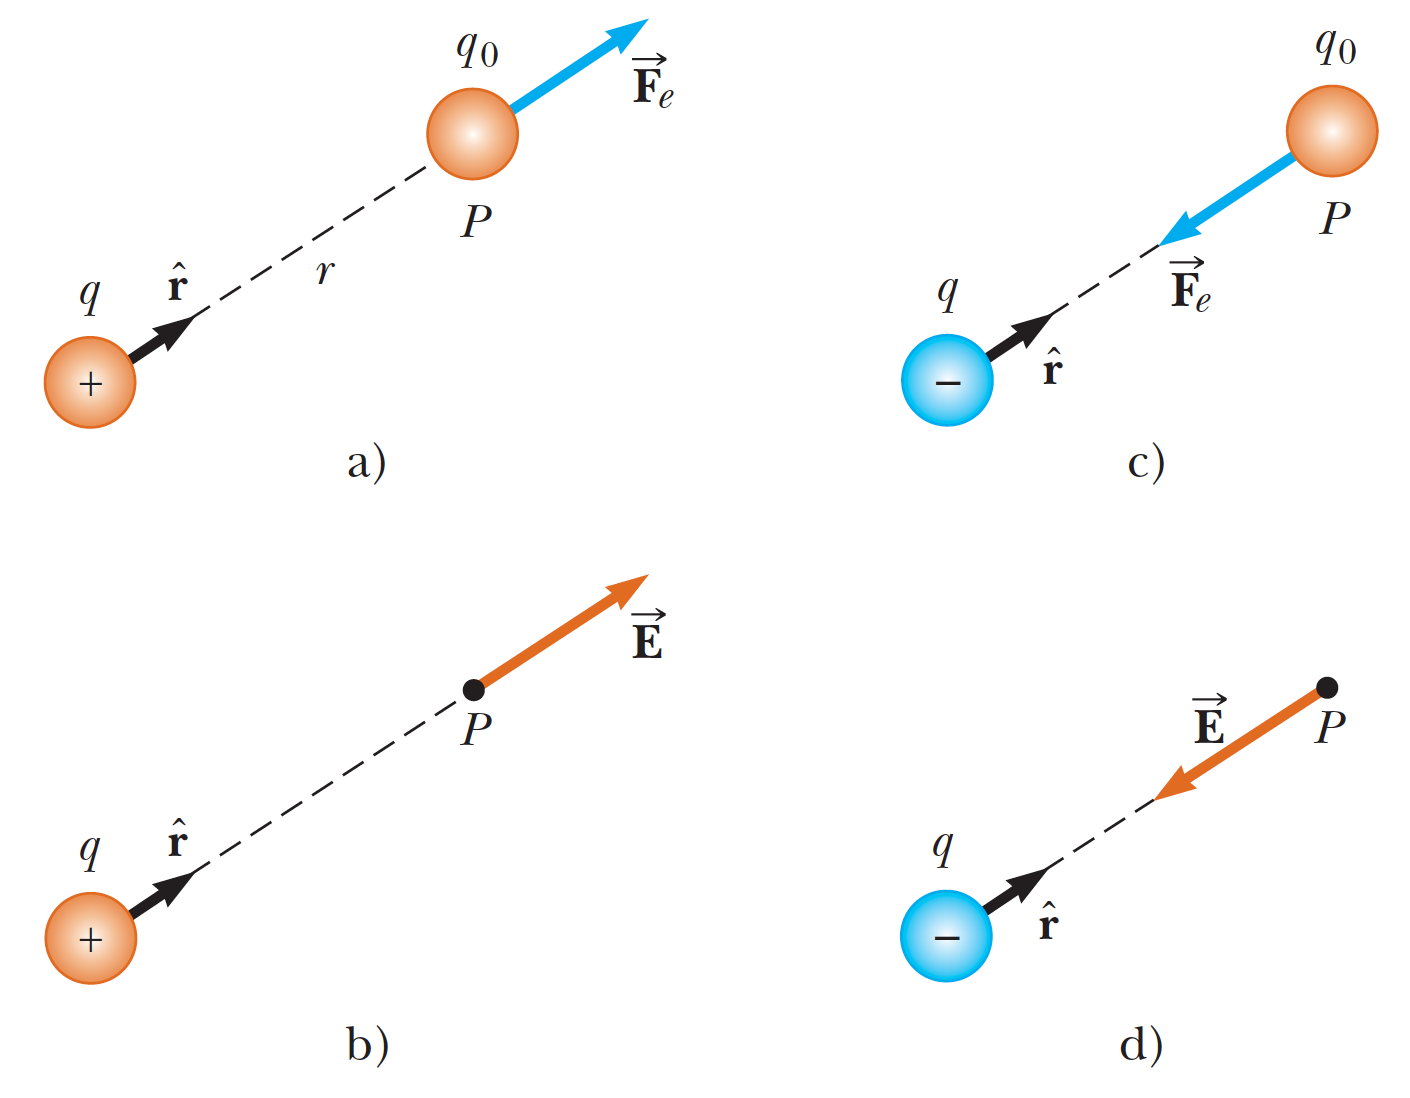
\includegraphics[width=0.45\textwidth]{4/figure_2}
      \caption{Una carga de prueba $q_{0}$ en el punto P está a una distancia $r$ de la carga puntual $q$.}
    \end{figure}

    \PN Ya que el campo eléctrico en P, que es la posición de la carga de prueba, queda definido por $\vec{E} = \vec{F}
    / q_{0}$, el campo eléctrico en P establecido por $q$ es
    \begin{equation*}
      \vec{E} = k \ \frac{q}{r^{2}} \ \hat{r}
    \end{equation*}

    \PN El campo eléctrico en el punto P debido a un grupo de cargas fuente se expresa como la suma vectorial
    \begin{equation*}
      \vec{E} = k \ \sum_{i} \frac{q_{i}}{r_{i}^{2}} \ \hat{r}_{i}
    \end{equation*}

    \PN donde $r_{i}$ es la distancia desde la i-ésima carga fuente $q_{i}$ hasta el punto P y $\hat{r}^{i}$ es un
    vector unitario dirigido de $q_{i}$ hacia P.

    \VS
    \PN \underline{Dipolo eléctrico:} se define como una carga positiva $q$ y una carga negativa $q$ separadas por una
    distancia $2d$. El dipolo eléctrico es un buen modelo de muchas moléculas. Los átomos y moléculas neutros se
    comportan como dipolos cuando se colocan en un campo eléctrico externo.

  \subsection{Campo eléctrico de una distribución de carga continua}
    \PN Con mucha frecuencia, en un grupo de cargas, la distancia existente entre ellas es mucho más reducida que la
    distancia entre el grupo y el punto donde se desea calcular el campo eléctrico. En esta situación, el sistema de
    cargas se modela como si fuera continuo. Es decir, el sistema de cargas espaciadas en forma compacta es equivalente
    a una carga total que es distribuida de forma continua a lo largo de alguna línea, sobre alguna superficie, o por
    todo el volumen.

    \VS El campo eléctrico en P debido a un elemento de carga con una carga $\Delta q$ es
    \begin{equation*}
      \Delta \vec{E} = k \ \frac{\Delta q}{r^{2}} \ \hat{r}
    \end{equation*}

    \PN donde $r$ es la distancia desde el elemento de carga hasta el punto P y $\hat{r}$ es el vector unitario
    dirigido desde el elemento de carga hasta P. El campo eléctrico total en P debido a todos los elementos en la
    distribución de carga es aproximadamente
    \begin{equation*}
      \vec{E} \approx k \ \sum_{i} \frac{\Delta q_{i}}{r_{i}^{2}} \ \hat{r}_{i}
    \end{equation*}

    \PN donde el índice $i$ se refiere al i-ésimo elemento de orden $i$ en la distribución. Ya que la distribución de
    carga ha sido modelada como continua, el campo total en P en el límite $\Delta q_{i} \rightarrow 0$ es
    \begin{equation*}
      \vec{E} = k \ \lim_{\Delta q_{i} \rightarrow 0} \ \sum_{i} \frac{\Delta q_{i}}{r_{i}^{2}} \ \hat{r}_{i} = k \ \int
      \ \frac{dq}{r^{2}} \ \hat{r}
    \end{equation*}

    \PN donde la integración es sobre toda la distribución de carga. La integración de la ecuación anterior es una
    operación vectorial y debe ser tratada en forma apropiada.

    \VS
    \PN Este tipo de cálculo se ilustra con varios ejemplos en los que la carga está distribuida a lo largo de una
    línea, sobre una superficie, o en todo un volumen. Cuando realice estos cálculos es conveniente que use el concepto
    de densidad de carga junto con las siguientes observaciones:
    \begin{itemize}
      \item Si una carga Q tiene una distribución uniforme en un volumen V, la \textbf{densidad de carga volumétrica}
      $\rho$ se define como
      \begin{equation*}
        \rho \equiv \frac{\text{Q}}{\text{V}}
      \end{equation*}

      \PN donde $rho$ está en C/$m^{3}$.

      \item Si una carga Q tiene una distribución uniforme sobre una superficie de área A, la \textbf{densidad de carga
      superficial} $\sigma$ se define como
      \begin{equation*}
        \sigma \equiv \frac{\text{Q}}{\text{A}}
      \end{equation*}

      \PN donde $sigma$ está en C/$m^{2}$.

      \item Si una carga Q tiene una distribución uniforme a lo largo de una línea de longitud $l$, la \textbf{densidad
      de carga lineal} $\lambda$ se define como
      \begin{equation*}
        \lambda \equiv \frac{\text{Q}}{l}
      \end{equation*}

      \PN donde $lambda$ está en C/$m$.

      \item Si la carga no tiene distribución uniforme en un volumen, superficie o línea, las cantidades de cargas $dq$
      en un elemento pequeño de volumen, superficie o longitud son
      \begin{equation*}
        dq = \rho \ d \text{V} \qquad dq = \sigma \ d \text{A} \qquad dq = \lambda \ dl
      \end{equation*}
    \end{itemize}

    \subsection{Líneas de campo eléctrico}
      \PN Una forma conveniente de visualizar los patrones de los campos eléctricos es el trazo de líneas conocidas
      como \textbf{líneas de campo eléctrico}, establecidas por primera vez por Faraday, las cuales relacionan el campo
      eléctrico con una región del espacio.

      \begin{figure}[H]
        \centering
        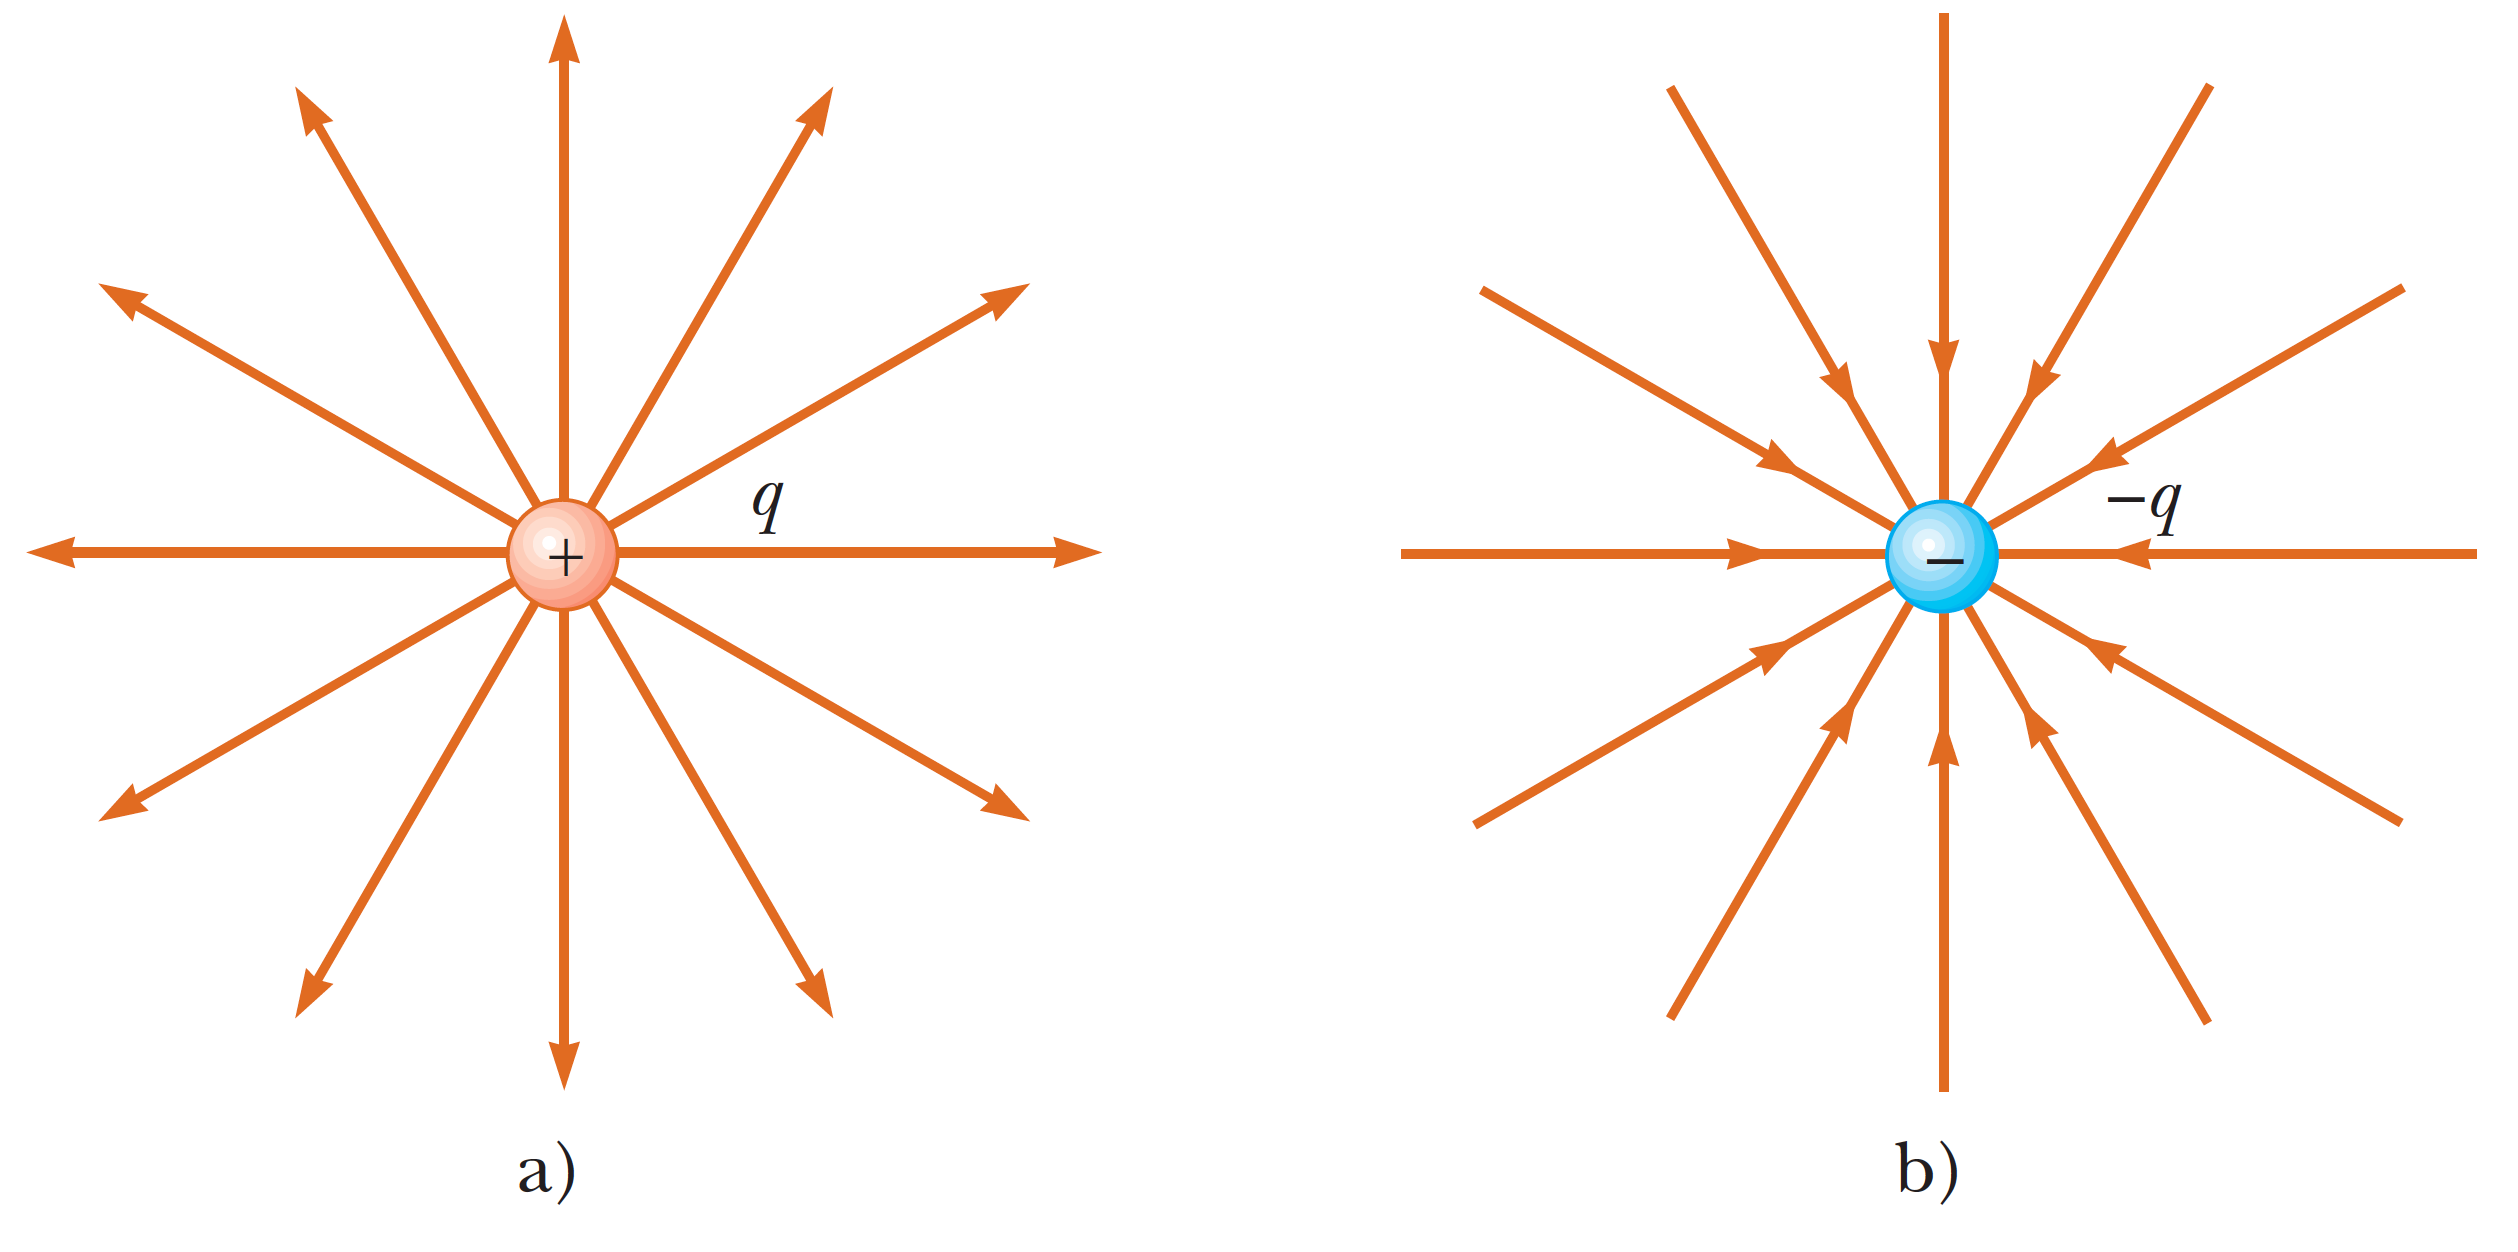
\includegraphics[width=0.6\textwidth]{4/figure_3}
        \caption{Líneas de campo eléctrico para una carga puntual.}

        \begin{multicols}{2}
          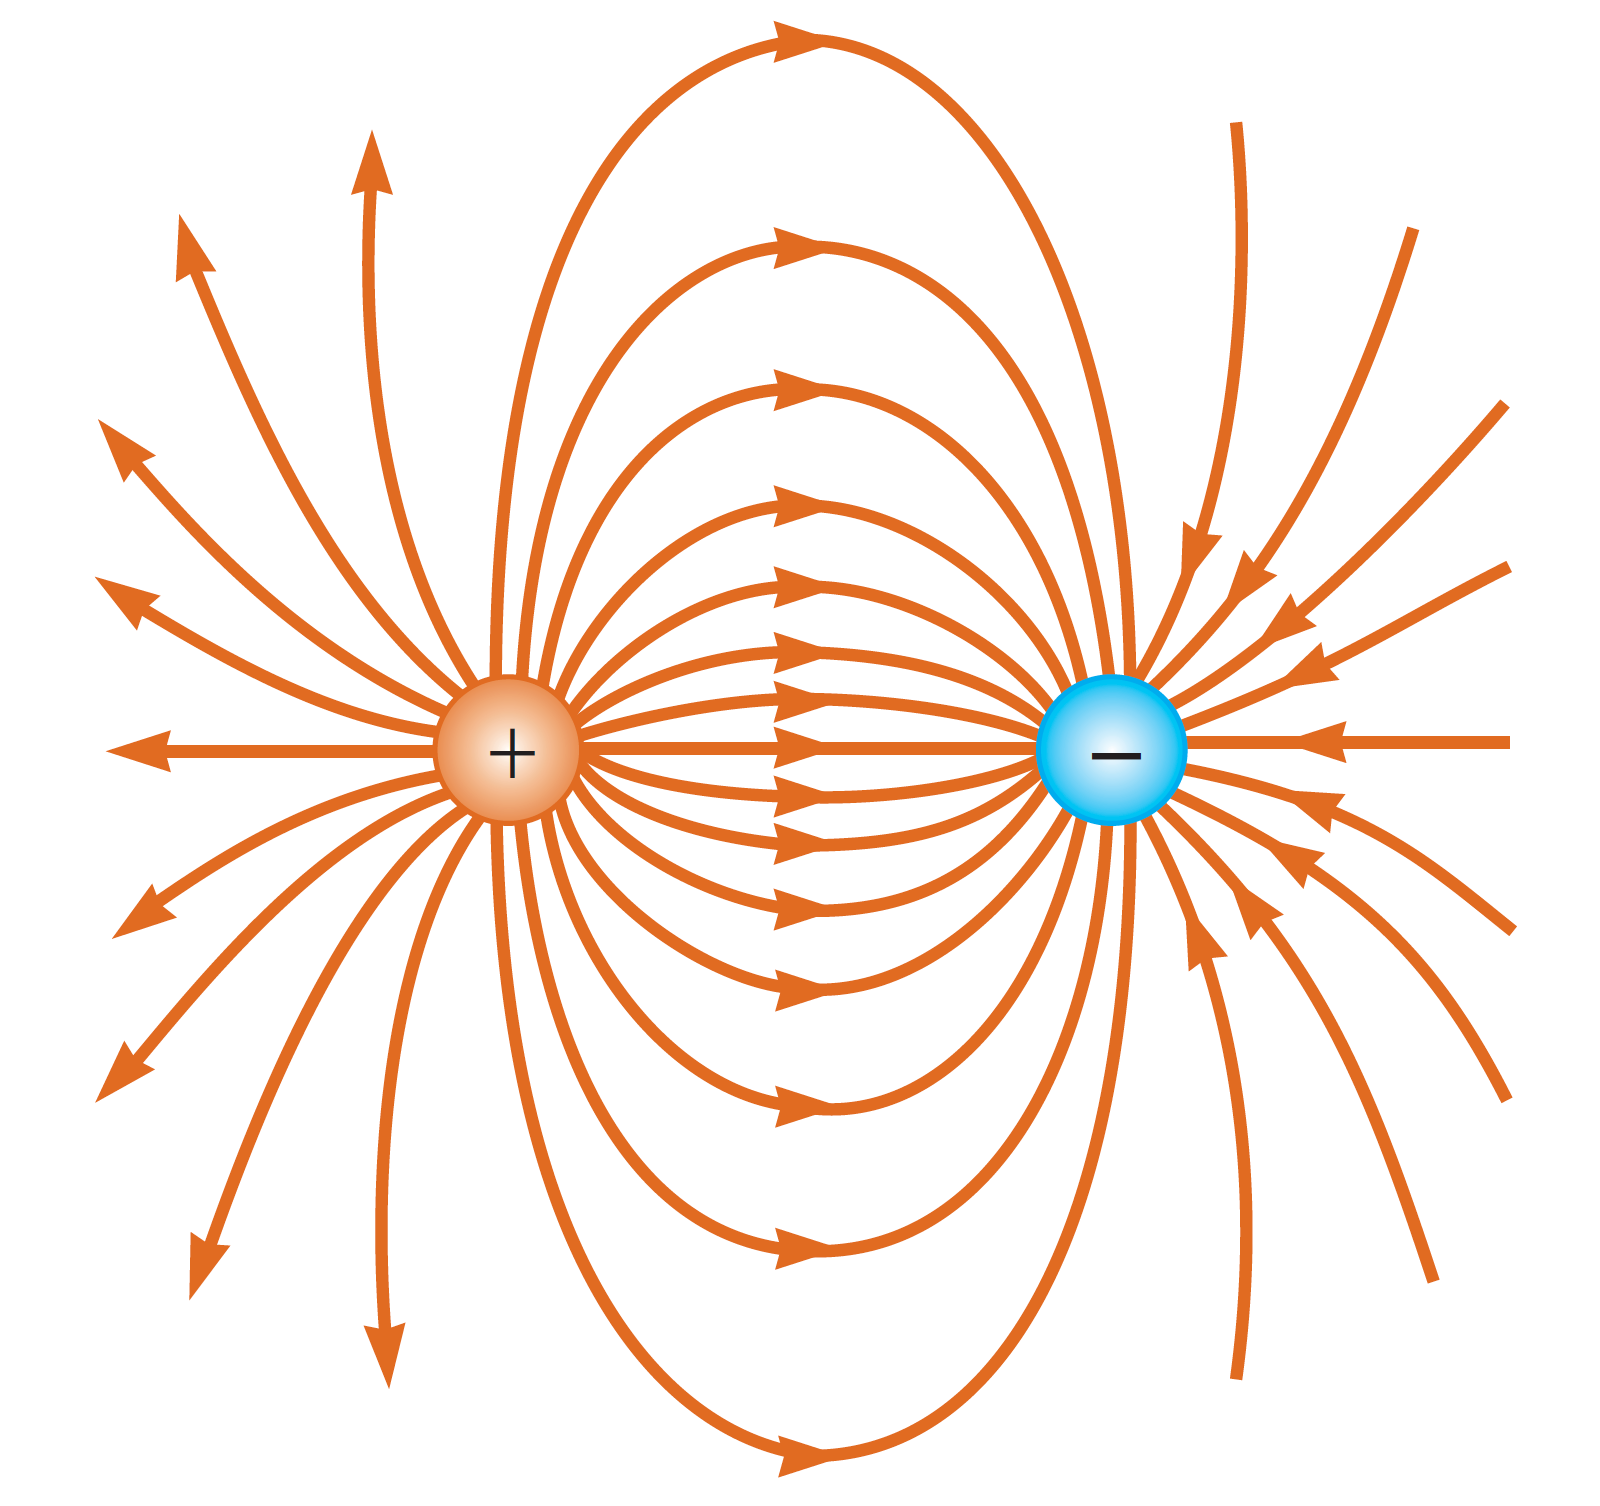
\includegraphics[width=0.3\textwidth]{4/figure_4}\par
          \caption{Líneas de campo eléctrico para dos cargas puntuales de igual magnitud y de signo opuesto.}
          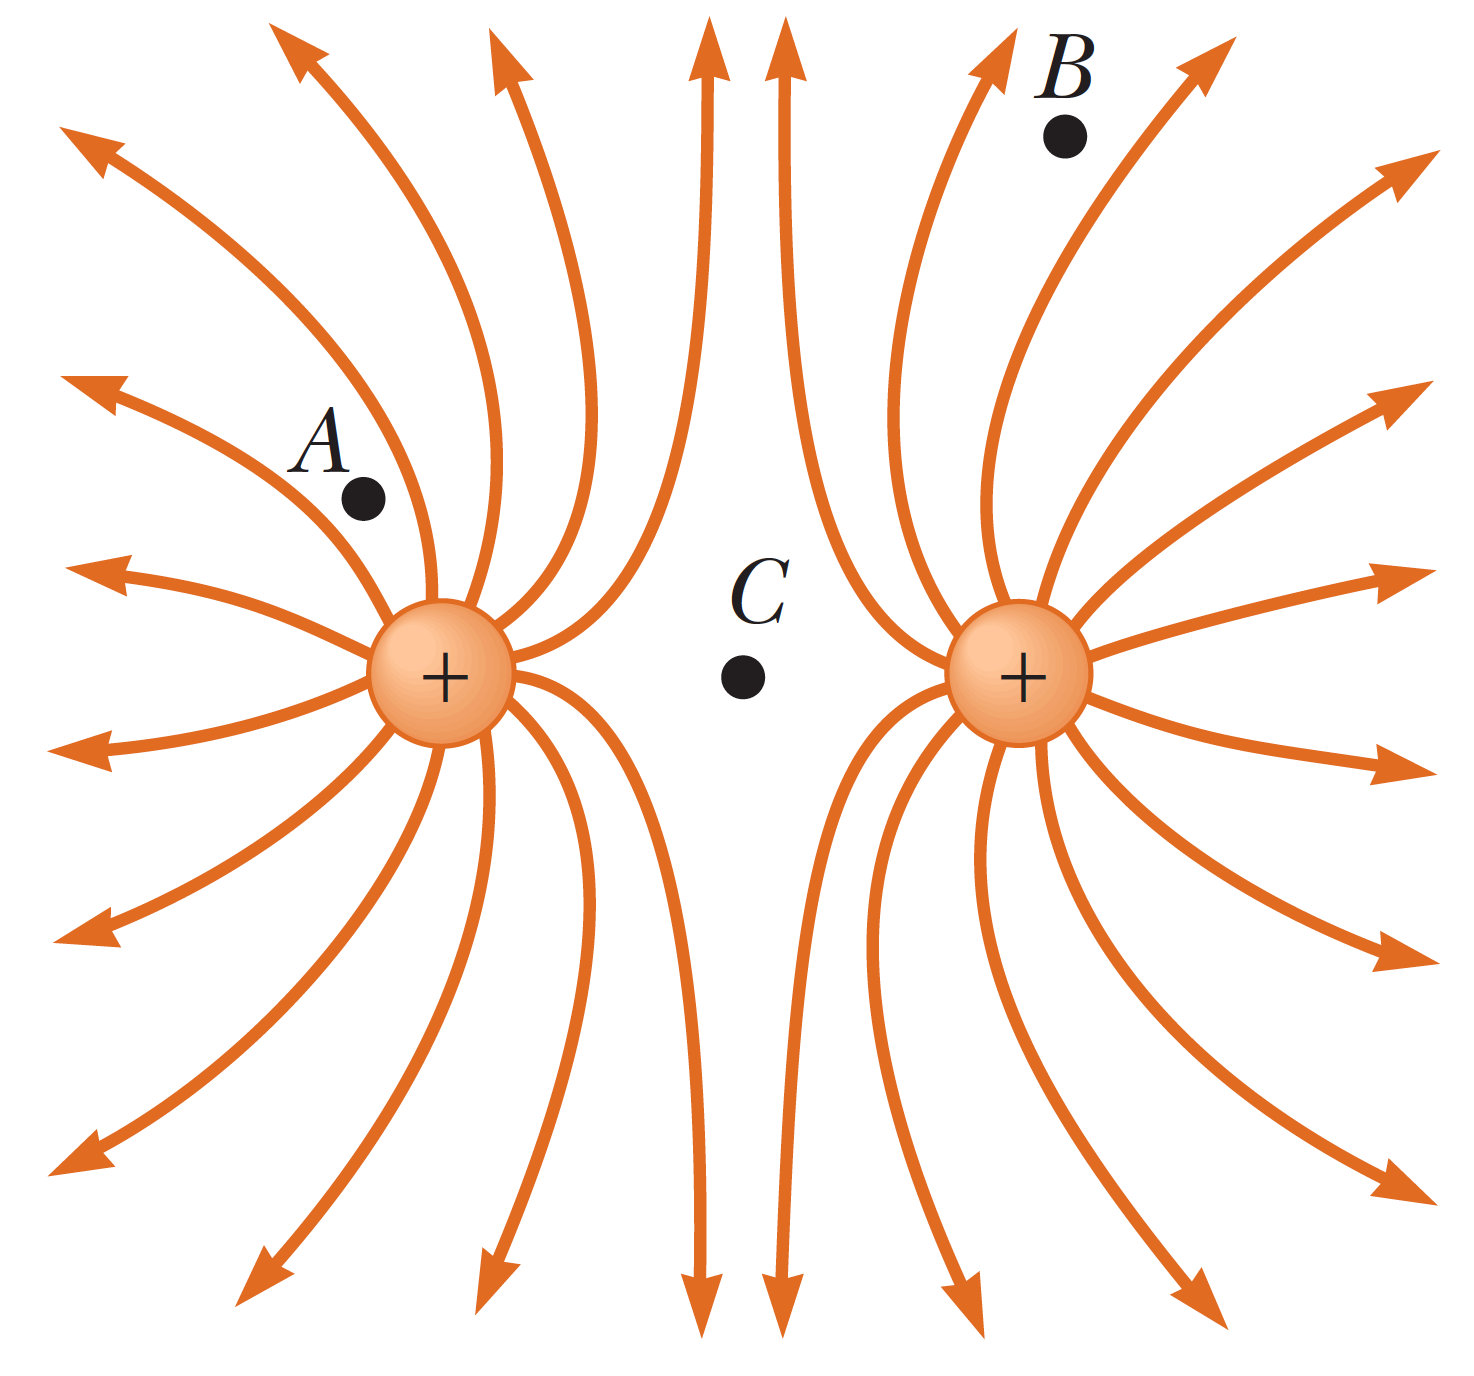
\includegraphics[width=0.3\textwidth]{4/figure_5}\par
          \caption{Líneas de campo eléctrico para dos cargas puntuales positivas.}
        \end{multicols}
      \end{figure}
